\documentclass[12pt, ]{article}

%\usepackage[top=1.5cm,bottom=1cm,left=2cm,right=2cm,a4paper]{geometry}
\usepackage{multirow}
\usepackage{url}
\usepackage{graphicx}
%\graphicspath{{path/}}

\title{Recognizing Differentially Expressed Genes in HCC}
\author{Javad Razvian}
\date{Aug 7, 2019}



\begin{document}
\maketitle

\section{Introduction}
The study's goal is to recognize special key genes in hepatocellular carcinoma (HCC) in response to the Question 1 available at \url{http://oncinfo.org/r_test}.
We have 8 control samples and 8 tissue samples given from Gene Expression Omnibus with access number GSE59259.
As the question asked, the differentially expressed genes (DEGs) between the HCCs and control samples were identified with the aid of limma
package in R with cutoff  adj.p.value~<~0.01. 

\section{Method}

The DEGs between HCC tumors and Liver-non neoplastic control were identified with 
limma \cite{bib:limma} package in R software. 
A small p-value (typically $\leq$ 0.05) indicates strong evidence against the null hypothesis, concluding that a significant difference does exist in expressed gene. The cutoff criterion was adjusted p-value < 0.01. 

We also repeated the analysing stage with another cutoff as other studies like \cite{bib:skg} suggest. This measure called log2 fold change (logFC) describing how much a quantity changes going from an initial to a final value. Postive value shows increment and negative value indicates decrement.
Therefore, we chose ``adjusted p-value < 0.01 and (logFC)|~>~2.0" as another cutoff.
While with the former cutoff we found 1570 genes, with the latter 143 genes were identified. However, for top five DE genes, they are similar except for just 
one gene (see table~\ref{tab:topgen}).

Finally we used the Volcano plot to justify our work. The farther the genes go the to right or left, the more dysregulated they are. However, genes appear higher on the volcano plot show highly significant changes. Green points depict the genes that have desired criteria with respect to 
adjusted p-values and logFC. 
The top 5 DE genes are illustrated in red. 

\begin{figure}{!htbp}

\begin{minipage}{.48\textwidth}
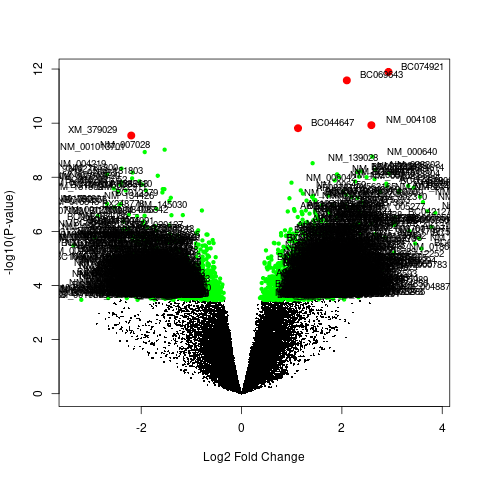
\includegraphics[width=\textwidth]{VolcanoPlotadj.png}
\scriptsize\centerline{adj.P.Value < 0.01}
\end{minipage}\hfill
\begin{minipage}{.48\textwidth}
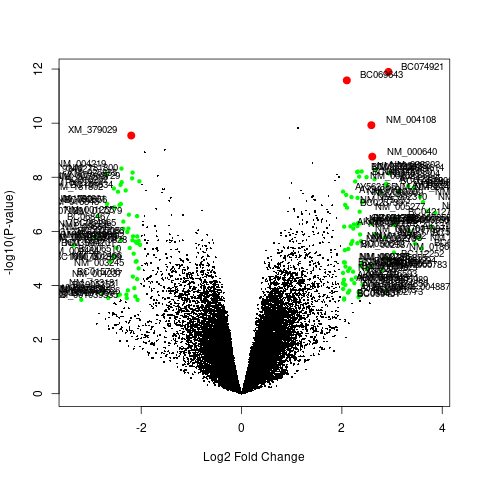
\includegraphics[width=\textwidth]{VolcanoPlotadjlogFC.png}
\scriptsize\centerline{adj.P.Value < 0.01 and |logFC|>2}
\end{minipage}
\caption{Volcano Plot}
\end{figure}

\section{Results}
The table~\ref{tab:topgen} depicts genes found as most frequent differentially expressed genes.

\begin{table}[!htbp]
\begin{tabular}{c||c|c}
    \multicolumn    {1}{c||}{cutoff criteria} & adj.P.Value < 0.01 & adj.P.Value < 0.01 \& |logFC|>2 \\\hline
    \multirow{5}{*}{\rotatebox{90}{genes}   } & BC074921 & BC074921\\
    & C069643 & BC069643\\
    & NM\_004108 & NM\_004108 \\
    & BC044647 & XM\_379029 \\
    & XM\_379029 & NM\_000640\\
\end{tabular}
    \caption{Top 5 DE genes}\label{tab:topgen}
\end{table}

    Figures~\ref{fig:heat1} and \ref{fig:heat2} show heatmap for both cutoff criteria.
    The maps show how the genes correlate with each others, and also cluster the genes based on their similarity in term of their expressions. 

\begin{figure}[!htbp]
    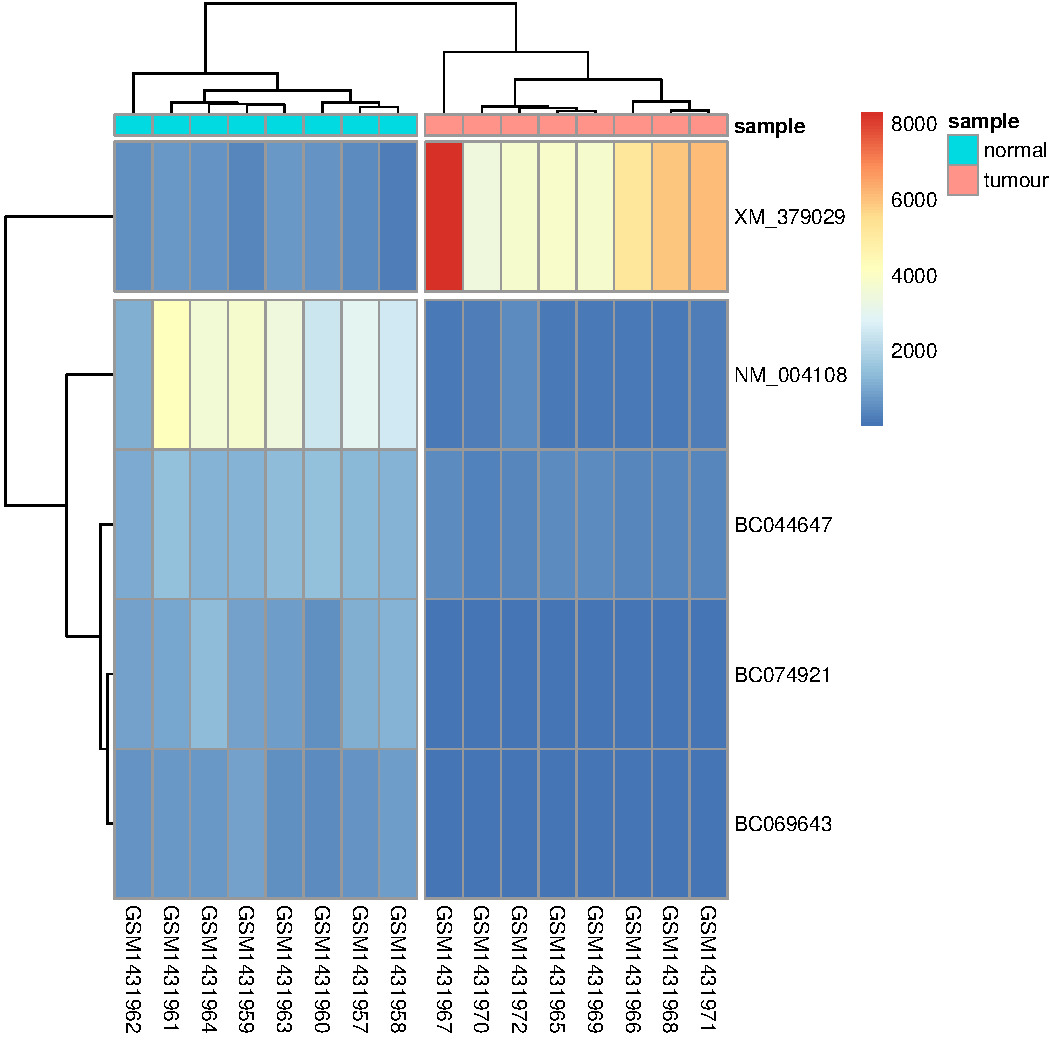
\includegraphics[width=\textwidth,]{heatmap-adj.pdf}
    \caption{Heatmap with cutoff ``adj.P.Value < 0.01''}
    \label{fig:heat1}
\end{figure}

\begin{figure}[!htbp]
    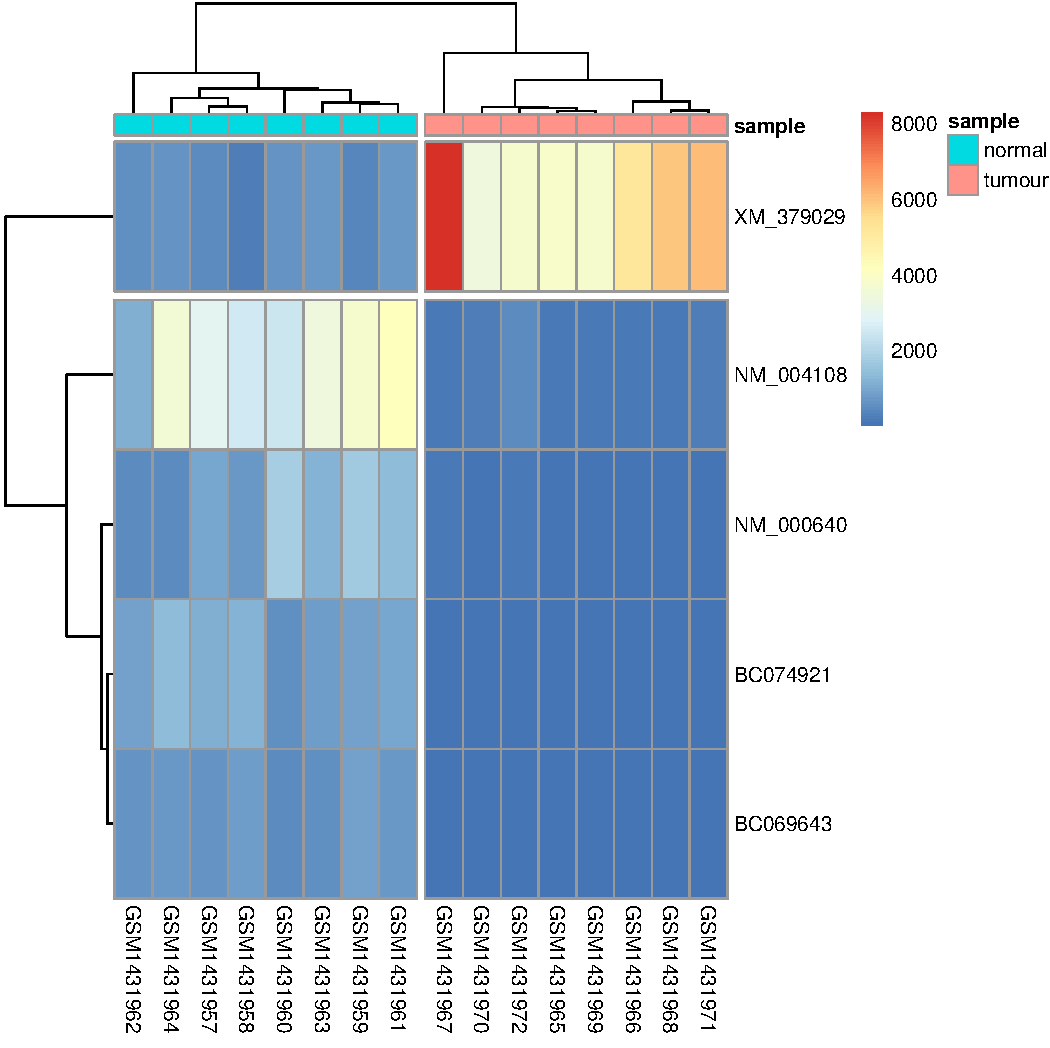
\includegraphics[width=\textwidth,]{heatmap-adjlogFC.pdf}
    \caption{Heatmap with cutoff ``adj.P.Value < 0.01 \& |logFC|>2''}
    \label{fig:heat2}
\end{figure}

\begin{thebibliography}{9}
    \bibitem {bib:skg} Zhang, X., Kang, C., Li, N., Liu, X., Zhang, J., Gao, F. and Dai, L., 2019. Identification of special key genes for alcohol-related hepatocellular carcinoma through bioinformatic analysis. PeerJ, 7, p.e6375.
    \bibitem {bib:limma} Ritchie, M. E., Phipson, B., Wu, D., Hu, Y., Law, C. W., Shi, W., \& Smyth, G. K. (2015). limma powers differential expression analyses for RNA-sequencing and microarray studies. Nucleic acids research, 43(7), e47-e47.
    \bibitem {} Microarray Data Analysis \url{https://discover.nci.nih.gov/microarrayAnalysis/Statistical.Tests.jsp}
    \bibitem {}   Gene Expression Omnibus \url{https://www.ncbi.nlm.nih.gov/geo/geo2r/?acc=GSE59259}
    \bibitem {}  Limma Tutorial, Available at \url{https://www.youtube.com/watch?v=Tg_qttx2koI&t=563s}.
    \bibitem {} Making a heatmap in R with the pheatmap package, Available at \url{https://davetang.org/muse/2018/05/15/making-a-heatmap-in-r-with-the-pheatmap-package/}.
    \bibitem {} Using Volcano Plots in R to Visualize Microarray and RNA-seq Results, Available at \url{https://www.gettinggeneticsdone.com/2014/05/r-volcano-plots-to-visualize-rnaseq-microarray.html}


%    \bibitem {}
\end{thebibliography}
\end{document}
